\chapter{Monitorización y Feedback Loop}
\label{cap:monitorizacion}

\section{Introducción}
\label{sec:intro_monitorizacion}

El despliegue de un modelo de \textit{Machine Learning} en producción no es el final del proceso, sino el inicio de su mantenimiento continuo. Un modelo puede degradarse gradualmente cuando la distribución de los datos reales se aleja de la distribución de entrenamiento (fenómeno conocido como \textbf{\textit{data drift}}) sin que ningún error de código lo evidencie. Este capítulo describe la capa de monitorización del sistema \textit{CORE-MP}, compuesta por métricas operativas con \textbf{Prometheus} y \textbf{Grafana}, detección de drift con \textbf{Evidently}, un feedback loop automatizado con \textbf{Apache Airflow} y alertas vía \textbf{Telegram}. El conjunto forma un ciclo de \textit{Continuous Training} (CT) autónomo que mantiene la calidad del modelo en producción sin intervención manual.

\section{Arquitectura de Monitorización}
\label{sec:arquitectura_monitorizacion}

La capa de monitorización amplía el sistema del despligue y puesta en producción con cuatro contenedores adicionales, todos orquestados en \texttt{docker-compose.yml}:

\begin{table}[H]
\centering
\footnotesize
\begin{tabular}{lllp{5cm}}
\hline
\textbf{Contenedor} & \textbf{Imagen} & \textbf{Puerto} & \textbf{Función} \\ \hline
\texttt{api}         & \texttt{Dockerfile.api}      & 8000 & Inferencia + exportación de métricas \\
\texttt{prometheus}  & \texttt{prom/prometheus}      & 9092 & Recolección y almacenamiento de métricas \\
\texttt{grafana}     & \texttt{grafana/grafana}      & 3000 & Visualización y alertas \\
\texttt{pushgateway} & \texttt{prom/pushgateway}     & 9091 & Métricas \textit{batch} del DAG de Airflow \\
\texttt{airflow}     & \texttt{apache/airflow:2.9.0} & 8080 & Orquestación del feedback loop \\
\texttt{train}       & \texttt{Dockerfile.train}     & ---  & Reentrenamiento (on-demand) \\ \hline
\end{tabular}
\caption{Contenedores del stack de monitorización de CORE-MP.}
\label{tab:contenedores_monitoring}
\end{table}

La Figura~\ref{fig:arquitectura_monitoring} muestra el flujo de información: Prometheus \textit{escrapea} la API cada 15~segundos; el DAG de Airflow empuja sus métricas de drift al Pushgateway, que Prometheus también recolecta; Grafana consume ambas fuentes en un \textit{dashboard} unificado.

\begin{figure}[H]
\centering
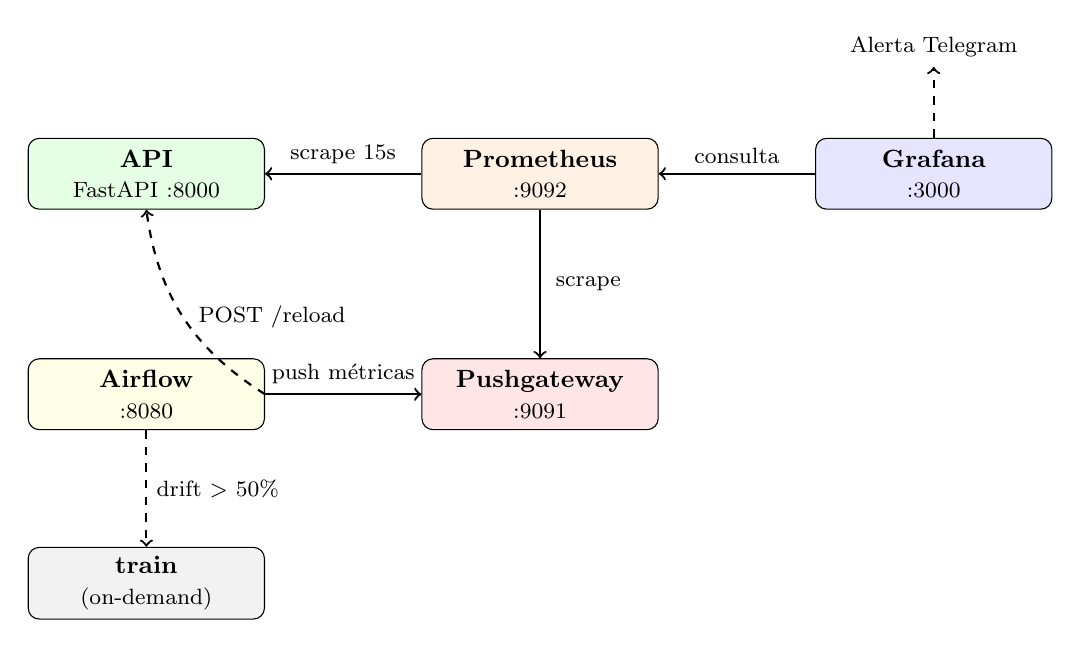
\begin{tikzpicture}[
    box/.style={rectangle, draw, rounded corners, minimum width=3cm, minimum height=0.9cm, align=center, font=\small},
    arrow/.style={->, thick},
    darrow/.style={->, thick, dashed}
]
    \node[box, fill=green!10]  (api)     at (0, 0)    {\textbf{API}\\\footnotesize FastAPI :8000};
    \node[box, fill=orange!10] (prom)    at (5, 0)    {\textbf{Prometheus}\\\footnotesize :9092};
    \node[box, fill=blue!10]   (grafana) at (10, 0)   {\textbf{Grafana}\\\footnotesize :3000};

    \node[box, fill=yellow!10] (airflow) at (0, -2.8) {\textbf{Airflow}\\\footnotesize :8080};
    \node[box, fill=red!10]    (pushgw)  at (5, -2.8) {\textbf{Pushgateway}\\\footnotesize :9091};
    \node[box, fill=gray!10]   (train)   at (0, -5.2) {\textbf{train}\\\footnotesize (on-demand)};

    \draw[arrow] (prom)    -- node[above]{\footnotesize scrape 15s}    (api);
    \draw[arrow] (grafana) -- node[above]{\footnotesize consulta}      (prom);
    \draw[arrow] (airflow) -- node[above]{\footnotesize push métricas} (pushgw);
    \draw[arrow] (prom)    -- node[right, xshift=2pt]{\footnotesize scrape} (pushgw);
    \draw[darrow] (airflow) -- node[right]{\footnotesize drift $>$ 50\%} (train);
    \draw[darrow] (airflow.east) to[bend left=25]
        node[right, xshift=2pt]{\footnotesize POST /reload} (api.south);
    \draw[darrow] (grafana.north) -- ++(0, 0.9)
        node[above]{\footnotesize Alerta Telegram};
\end{tikzpicture}
\caption{Flujo de datos del stack de monitorización. Flechas sólidas: métricas; discontinuas: acciones de control del feedback loop.}
\label{fig:arquitectura_monitoring}
\end{figure}

\section{Métricas Operativas y Dashboard}
\label{sec:metricas_operativas}

La API instrumenta todas las rutas HTTP mediante \texttt{prometheus-fastapi-instrumentator}, que expone histogramas de latencia y contadores de peticiones en \texttt{GET /metrics/prometheus}. Adicionalmente, se define el contador personalizado \texttt{predictions\_total}, etiquetado por resultado (\texttt{compatible=true/false}), y el módulo \texttt{src/monitor/service.py} mantiene un \texttt{MetricsTracker} \textit{thread-safe} (con \texttt{threading.Lock}) que calcula la latencia media acumulada:

\begin{equation}
\bar{L} = \frac{\displaystyle\sum_{i=1}^{N} \bigl(t_{\text{respuesta},i} - t_{\text{solicitud},i}\bigr)}{N}
\label{eq:latencia_media}
\end{equation}

Grafana se provisiona automáticamente desde \texttt{monitoring/grafana/provisioning/} con un \textit{dashboard} de refresco de 10~segundos y cuatro paneles (Tabla~\ref{tab:grafana_paneles}). El umbral de P95 está fijado en 0{,}5~s: si se supera, el panel se colorea en rojo. Para garantizar la idempotencia del provisioning, el \textit{datasource} de Prometheus tiene un UID fijo (\texttt{uid: prometheus}), de modo que los paneles encuentran su fuente de datos incluso tras recrear el contenedor de Grafana.

\begin{table}[H]
\centering
\footnotesize
\begin{tabular}{llp{7cm}}
\hline
\textbf{Panel} & \textbf{Tipo} & \textbf{Consulta PromQL} \\ \hline
Request Rate (req/s)   & Serie temporal & \texttt{sum(rate(http\_request\_duration\_seconds\_count[1m]))} \\[4pt]
Latencia P95 (s)       & Serie temporal & \texttt{histogram\_quantile(0.95, sum by (le) (rate(\ldots[5m])))} \\[4pt]
Total predicciones     & Estadístico    & \texttt{predictions\_total} \\[4pt]
Tasa de errores 5xx    & Serie temporal & \texttt{sum(rate(\ldots\{status=\textasciitilde"5.."\}[1m]))} \\ \hline
\end{tabular}
\caption{Paneles del dashboard de Grafana para el sistema CORE-MP.}
\label{tab:grafana_paneles}
\end{table}

La Figura~\ref{fig:grafana_dashboard} muestra el dashboard en funcionamiento con tráfico real: el panel \textit{Request Rate} refleja las peticiones generadas durante la validación, \textit{Latencia P95} se mantiene en torno a 95~ms y el contador de predicciones acumula 70 llamadas sin errores 5xx.

\begin{figure}[H]
\centering
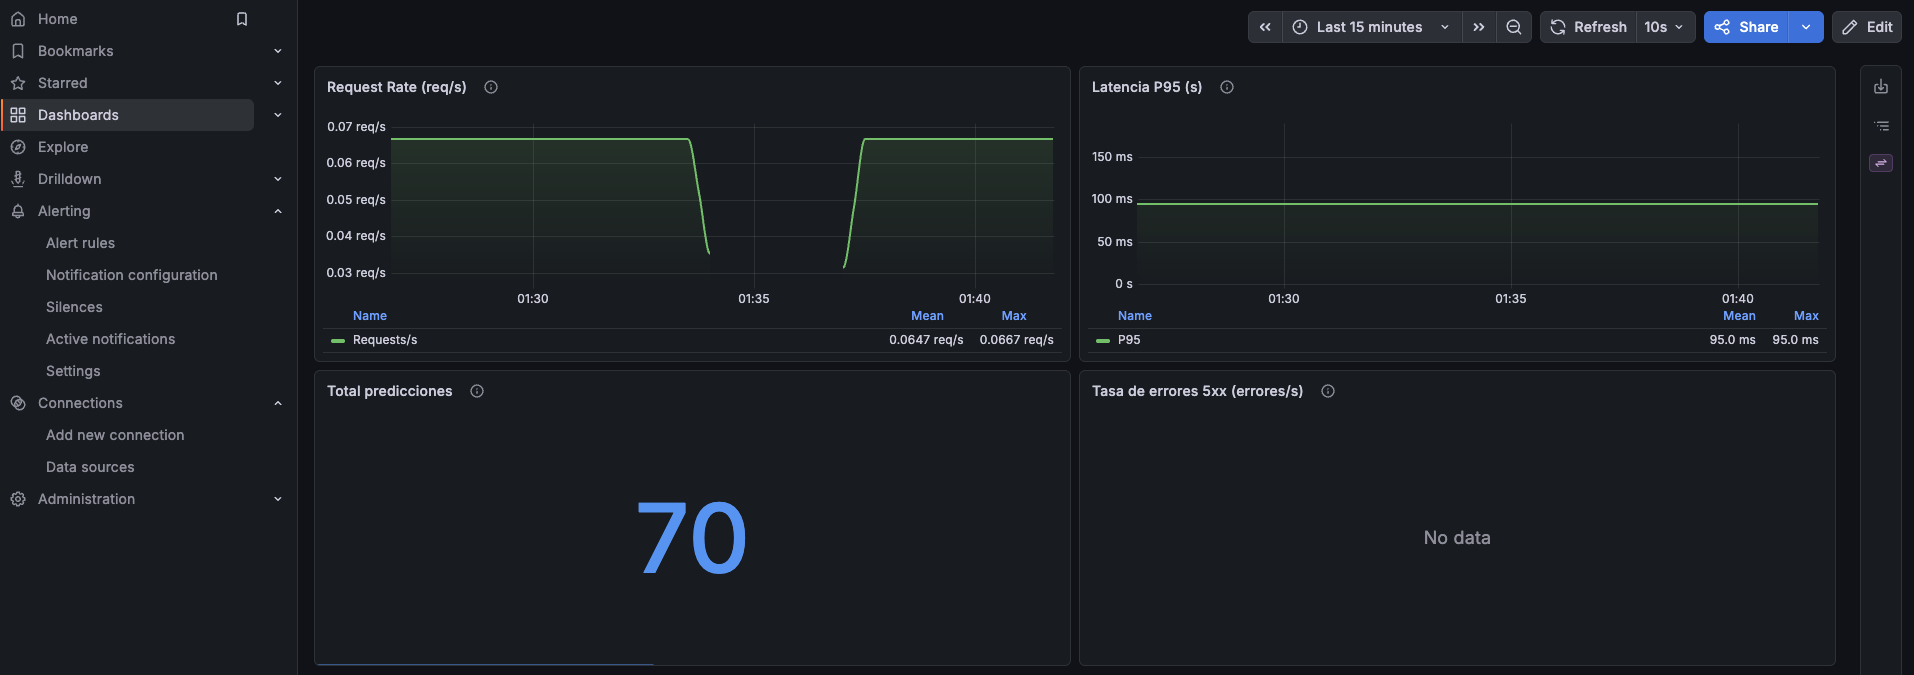
\includegraphics[width=0.82\textwidth]{Pictures/grafana_dashboard.png}
\caption{Dashboard de Grafana con los cuatro paneles de monitorización operativa de CORE-MP en tiempo real.}
\label{fig:grafana_dashboard}
\end{figure}

\section{Detección de Drift de Datos}
\label{sec:drift}

El \textbf{\textit{data drift}} se produce cuando la distribución de los datos de entrada en producción se aleja de la distribución de entrenamiento, degradando métricas como F1 o MAE aunque el código no tenga errores. La detección se implementa sobre seis características derivadas seleccionadas en el modelado:

\begin{itemize}
    \item \texttt{same\_love\_language}
    \item \texttt{ambition\_diff}
    \item \texttt{emotional\_expressiveness\_diff}
    \item \texttt{spontaneity\_diff}
    \item \texttt{overall\_match\_score}
    \item \texttt{personality\_distance\_sum}
\end{itemize}

Tras cada predicción, \texttt{src/monitor/drift\_logger.py} calcula estas seis features y las añade incrementalmente a \texttt{current\_traffic.csv}. Los datos de referencia (\texttt{reference\_data.csv}) se generan una única vez antes de la puesta en marcha, tomando 2.000 registros del \textit{dataset} original con las mismas fórmulas, para garantizar la comparabilidad.

La detección propiamente dicha la realiza \textbf{Evidently} mediante tests estadísticos (Kolmogorov-Smirnov para variables continuas, $\chi^2$ para categóricas). El análisis requiere al menos 50~muestras (\texttt{MIN\_SAMPLES~=~50}) para evitar resultados espurios. Si la proporción de features con drift supera el \textbf{50\%} (\texttt{DRIFT\_THRESHOLD~=~0.5}), se activa el reentrenamiento. En cualquier caso, se empujan dos métricas al Pushgateway (\texttt{core\_mp\_drift\_detected} y \texttt{core\_mp\_drift\_share}) para su visualización en Grafana.

\section{Feedback Loop con Airflow y Alertas}
\label{sec:feedback_loop}

El feedback loop se implementa como el DAG \texttt{core\_mp\_feedback\_loop} en Apache Airflow, con ejecución \textbf{horaria} y sin \textit{catchup}. Consta de tres tareas: \texttt{evaluate\_drift} (BranchPythonOperator) ejecuta el análisis de Evidently, empuja las métricas al Pushgateway y decide qué rama ejecutar; \texttt{retrain\_task} (PythonOperator) lanza \texttt{docker compose run --rm train} para reentrenar ambos modelos y llama a \texttt{POST /reload} para recargarlos en la API \textbf{sin reiniciar el servidor}; \texttt{skip\_task} (EmptyOperator) no realiza ninguna acción cuando no hay drift. La tarea de reentrenamiento tiene 1~reintento automático con 2~minutos de espera.

Las alertas de Grafana notifican al equipo vía \textbf{Telegram} configurando un \textit{contact point} \texttt{telegram-g5} como destino de la política de notificaciones por defecto. Se definen dos reglas de alerta (Figura~\ref{fig:alertas_grafana}):

\begin{itemize}
    \item \textbf{API caída:} se dispara cuando \texttt{up\{job="core\_mp\_api"\} < 1} se mantiene durante 1~minuto, indicando que Prometheus no puede alcanzar el endpoint de métricas de la API.
    \item \textbf{Latencia P95 alta:} se dispara cuando \texttt{histogram\_quantile(0.95, \ldots) > 0.5} se sostiene durante 2~minutos, señalando una posible degradación del servicio.
\end{itemize}

\begin{figure}[H]
\centering
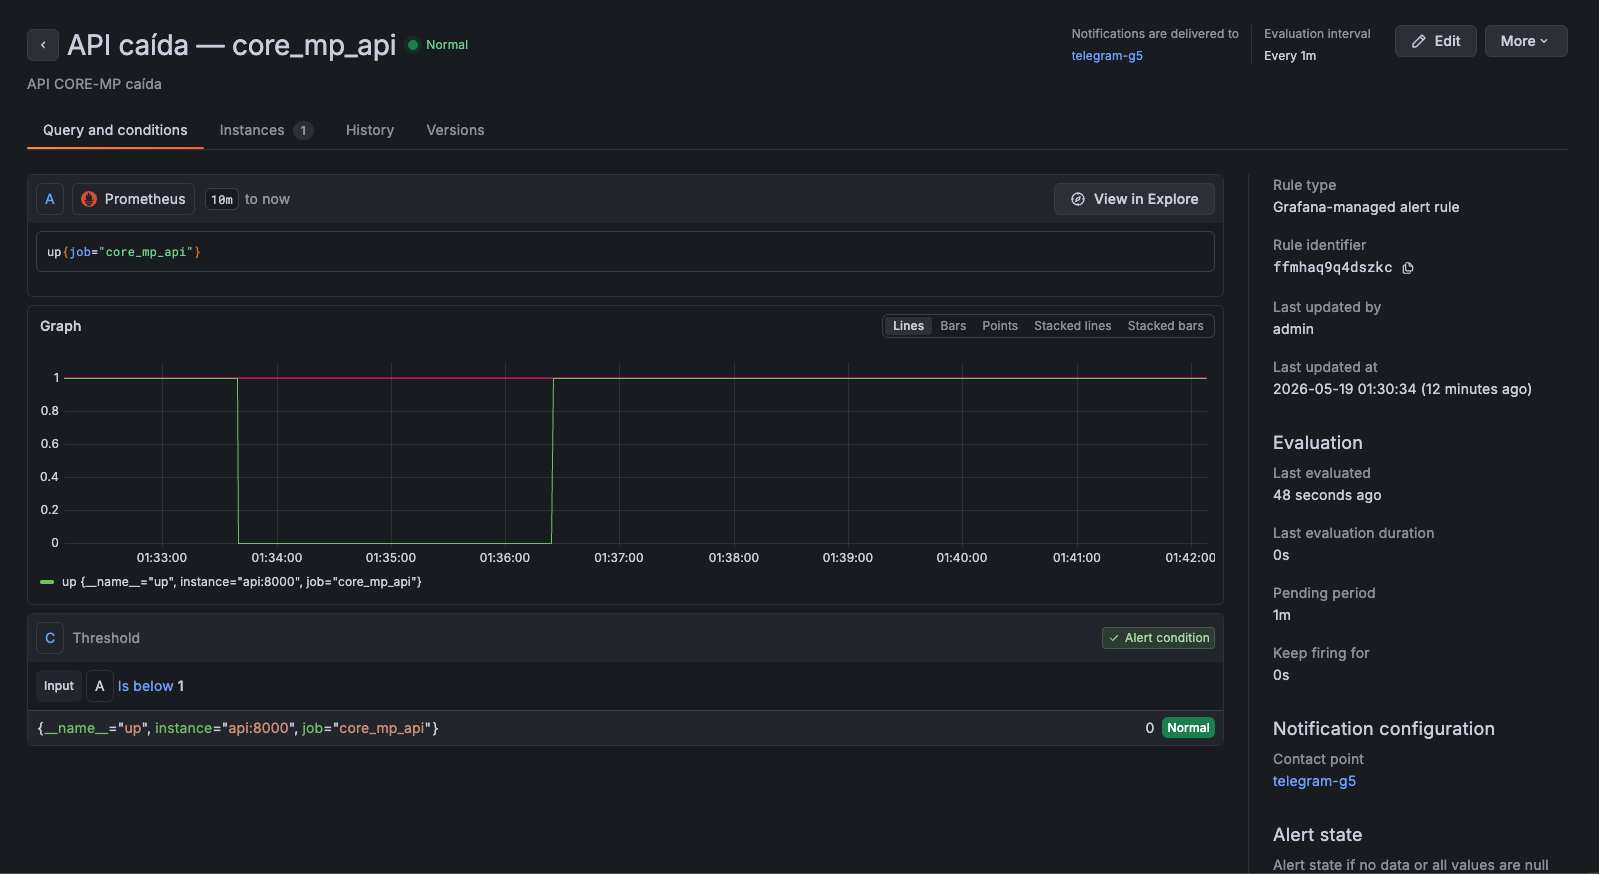
\includegraphics[width=0.48\textwidth]{Pictures/grafana_alerta_api_caida.png}
\hfill
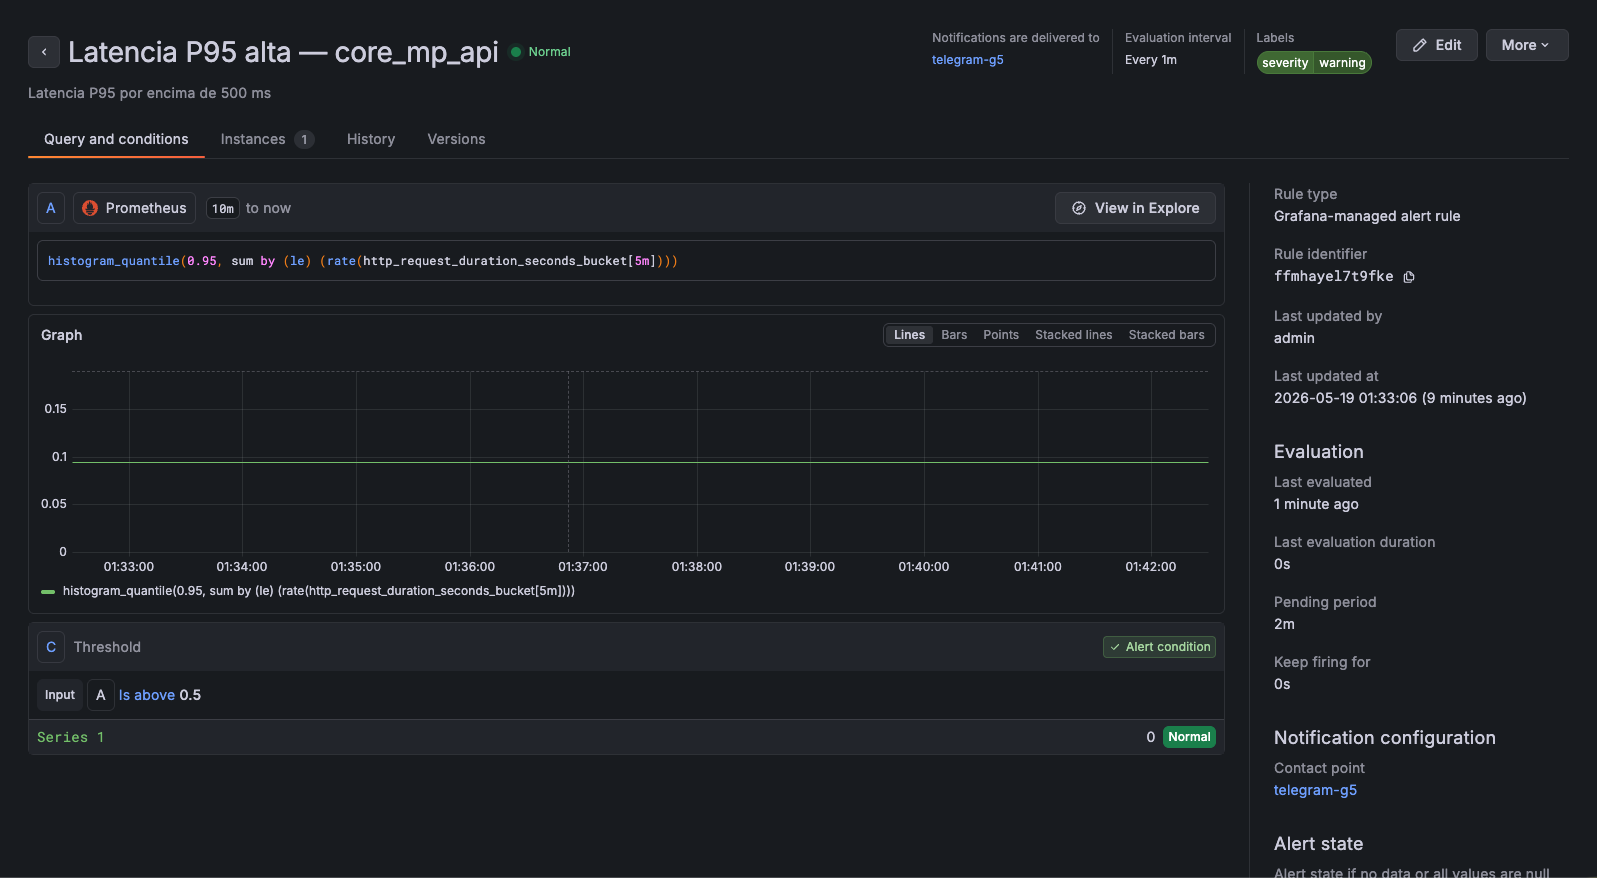
\includegraphics[width=0.48\textwidth]{Pictures/grafana_alerta_latencia.png}
\caption{Reglas de alerta en Grafana. Izquierda: ``API caída'' (consulta \texttt{up\{job="core\_mp\_api"\}}, umbral \textit{below}~1). Derecha: ``Latencia P95 alta'' (\texttt{histogram\_quantile(0.95,\,\ldots)}, umbral \textit{above}~0.5~s). Ambas notifican vía \textit{contact point} \texttt{telegram-g5}.}
\label{fig:alertas_grafana}
\end{figure}

La Figura~\ref{fig:grafana_contacts} muestra la pantalla de \textit{Contact points} de Grafana con el canal \texttt{telegram-g5} activo, usado por 1 política de notificación y 2 reglas de alerta. La validación end-to-end se realizó deteniendo el contenedor de la API (\texttt{docker compose stop api}) y verificando la recepción de los mensajes \textbf{FIRING} y \textbf{RESOLVED} en el grupo de Telegram del equipo (Figura~\ref{fig:telegram_alertas}).

\begin{figure}[H]
\centering
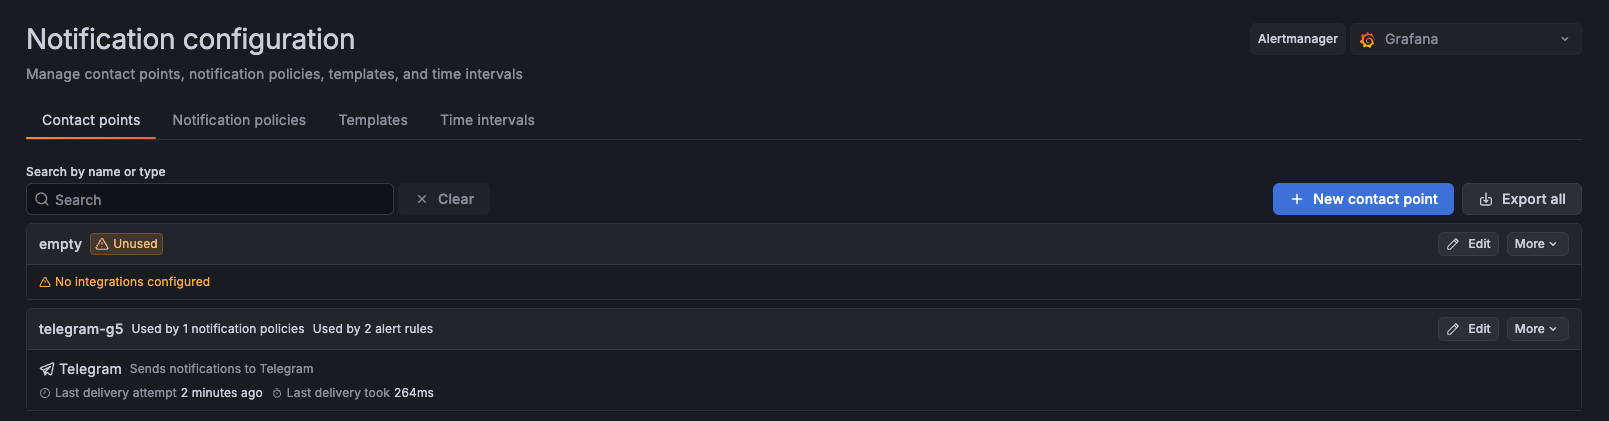
\includegraphics[width=0.7\textwidth]{Pictures/grafana_contact_points.png}
\caption{Pantalla de \textit{Contact points} de Grafana: el canal \texttt{telegram-g5} aparece asociado a 1 política de notificación y 2 reglas de alerta, con última entrega hace 2 minutos.}
\label{fig:grafana_contacts}
\end{figure}

\begin{figure}[H]
\centering
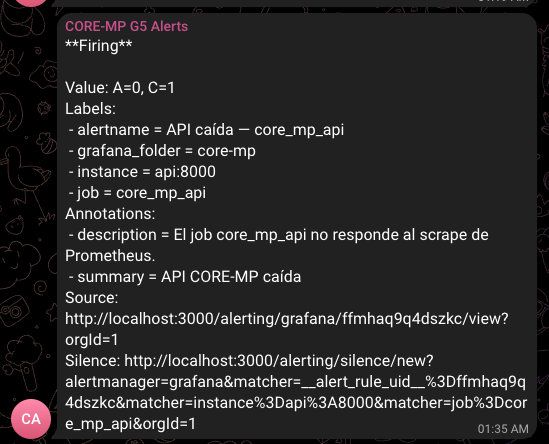
\includegraphics[width=0.34\textwidth]{Pictures/telegram_firing.png}
\hspace{0.04\textwidth}
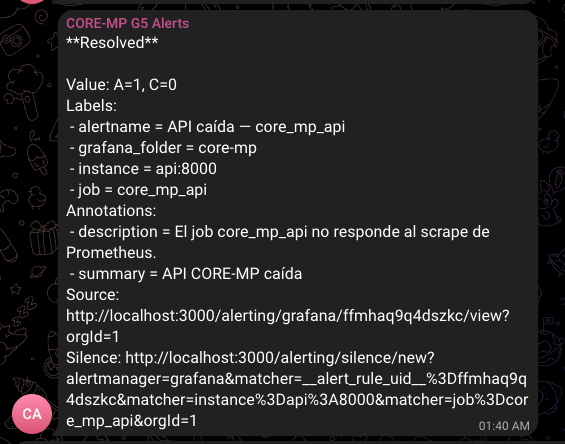
\includegraphics[width=0.34\textwidth]{Pictures/telegram_resolved.png}
\caption{Ciclo completo de alerta vía Telegram: mensaje \textbf{FIRING} (izquierda) al caer la API y \textbf{RESOLVED} (derecha) al recuperarse, ~1~min después.}
\label{fig:telegram_alertas}
\end{figure}

\section{Ciclo de Vida del Modelo}
\label{sec:ciclo_vida}

La Figura~\ref{fig:ciclo_vida} integra todos los componentes en una visión global del ciclo autónomo del modelo \textit{CORE-MP}.

\begin{figure}[H]
\centering
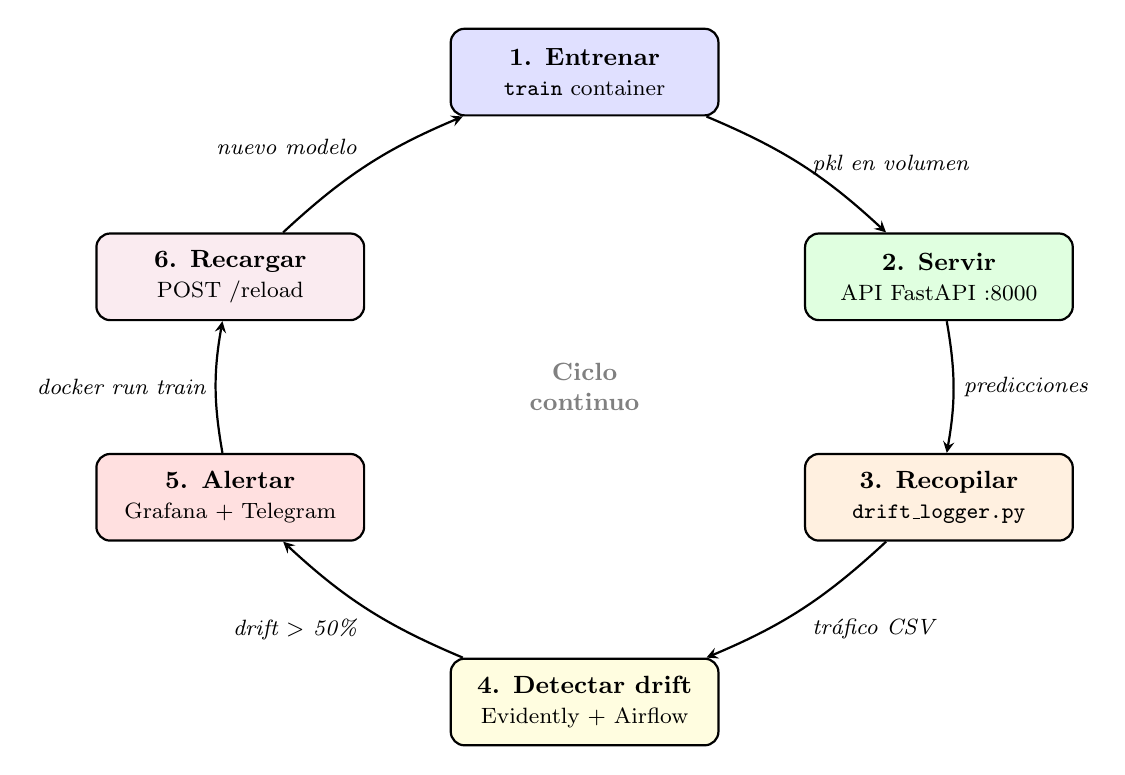
\begin{tikzpicture}[
    lifestep/.style={rectangle, draw, rounded corners=5pt, minimum width=3.4cm,
                 minimum height=1.1cm, align=center, font=\small, thick},
    arrow/.style={->, thick, >=stealth},
    lbl/.style={font=\footnotesize\itshape, midway}
]
    \node[lifestep, fill=blue!12]   (train)   at (0,     4)    {\textbf{1. Entrenar}\\\footnotesize \texttt{train} container};
    \node[lifestep, fill=green!12]  (serve)   at (4.5,   1.4)  {\textbf{2. Servir}\\\footnotesize API FastAPI :8000};
    \node[lifestep, fill=orange!12] (collect) at (4.5,  -1.4)  {\textbf{3. Recopilar}\\\footnotesize \texttt{drift\_logger.py}};
    \node[lifestep, fill=yellow!12] (detect)  at (0,    -4)    {\textbf{4. Detectar drift}\\\footnotesize Evidently + Airflow};
    \node[lifestep, fill=red!12]    (alert)   at (-4.5, -1.4)  {\textbf{5. Alertar}\\\footnotesize Grafana + Telegram};
    \node[lifestep, fill=purple!8]  (reload)  at (-4.5,  1.4)  {\textbf{6. Recargar}\\\footnotesize POST /reload};

    \draw[arrow] (train)   to[bend left=10] node[lbl, right]{pkl en volumen}   (serve);
    \draw[arrow] (serve)   to[bend left=10] node[lbl, right]{predicciones}     (collect);
    \draw[arrow] (collect) to[bend left=10] node[lbl, below right]{tráfico CSV} (detect);
    \draw[arrow] (detect)  to[bend left=10] node[lbl, below left]{drift $>$ 50\%} (alert);
    \draw[arrow] (alert)   to[bend left=10] node[lbl, left]{docker run train}  (reload);
    \draw[arrow] (reload)  to[bend left=10] node[lbl, above left]{nuevo modelo} (train);

    \node[font=\small\bfseries, gray, align=center] at (0,0) {Ciclo\\continuo};
\end{tikzpicture}
\caption{Ciclo de vida continuo del modelo CORE-MP: las predicciones alimentan la detección de drift, que activa el reentrenamiento y la recarga sin interrumpir el servicio.}
\label{fig:ciclo_vida}
\end{figure}

\section{Conclusiones}
\label{sec:conclusiones_monitorizacion}

La implementación de este hito transforma \textit{CORE-MP} en un sistema MLOps de madurez avanzada. Sus tres aportaciones principales son:

\begin{enumerate}
    \item \textbf{Observabilidad completa:} métricas operativas (latencia P95, tasa de peticiones, errores 5xx) y métricas de calidad del modelo (drift de datos) confluyen en un \textit{dashboard} unificado en Grafana, con alertas proactivas vía Telegram.

    \item \textbf{Detección y respuesta automática al drift:} Evidently identifica cambios en la distribución de entrada antes de que se manifiesten como errores perceptibles; Airflow cierra el bucle reentrenando el modelo y recargando la API sin interrupción del servicio.

    \item \textbf{Infraestructura como código:} toda la pila (\texttt{docker-compose.yml}, provisioning de Grafana y DAG de Airflow) se define como código, permitiendo reproducir el entorno completo con un único comando.
\end{enumerate}
